% Template for Cogsci submission with R Markdown

% Stuff changed from original Markdown PLOS Template
\documentclass[10pt, letterpaper]{article}

\usepackage{cogsci}
\usepackage{pslatex}
\usepackage{float}
\usepackage{caption}

% amsmath package, useful for mathematical formulas
\usepackage{amsmath}

% amssymb package, useful for mathematical symbols
\usepackage{amssymb}

% hyperref package, useful for hyperlinks
\usepackage{hyperref}

% graphicx package, useful for including eps and pdf graphics
% include graphics with the command \includegraphics
\usepackage{graphicx}

% Sweave(-like)
\usepackage{fancyvrb}
\DefineVerbatimEnvironment{Sinput}{Verbatim}{fontshape=sl}
\DefineVerbatimEnvironment{Soutput}{Verbatim}{}
\DefineVerbatimEnvironment{Scode}{Verbatim}{fontshape=sl}
\newenvironment{Schunk}{}{}
\DefineVerbatimEnvironment{Code}{Verbatim}{}
\DefineVerbatimEnvironment{CodeInput}{Verbatim}{fontshape=sl}
\DefineVerbatimEnvironment{CodeOutput}{Verbatim}{}
\newenvironment{CodeChunk}{}{}

% cite package, to clean up citations in the main text. Do not remove.
\usepackage{apacite}

% KM added 1/4/18 to allow control of blind submission


\usepackage{color}

% Use doublespacing - comment out for single spacing
%\usepackage{setspace}
%\doublespacing


% % Text layout
% \topmargin 0.0cm
% \oddsidemargin 0.5cm
% \evensidemargin 0.5cm
% \textwidth 16cm
% \textheight 21cm

\title{Modeling Selection in Active Cross-situational Word Learning}


\author{{\large \bf George~Kachergis (kachergis@stanford.edu)} \\ Department of Psychology, Stanford University \\ Stanford, CA \AND {\large \bf Martin~Zettersten (mzettersten@ucsd.edu)} \\ Department of Cognitive Science, University of California, San Diego \\ San Diego, CA}


\begin{document}

\maketitle

\begin{abstract}
Word learning is a complex process, influenced not only by the words and
referents in the language environment, but also by what learners
selectively attend to, which in turn is likely determined by their prior
knowledge.

\textbf{Keywords:}
active learning; cross-situational word learning; self-directed
learning; uncertainty reduction
\end{abstract}

\section{Introduction}\label{introduction}

Early word learning is often thought of as largely determined by the
learners' linguistic environment, where they can only learn what is
present in the input. Increasingly, research is finding that
learners--even at a young age--are involved in selecting and shaping
their input, and that such self-directed, active learning can accelerate
acquisition. Understanding the strategies that learners of all ages use
to shape their experience will help us build and improve theories of
language acquisition. It can also help us understand what cognitive
mechanisms and strategies learners are able to deploy, and consequently
enable us to design curricula that better match their expanding
capabilities. For example, although the classic conceptual @hunter1988
model posits that infants have preferences for both novel and familiar
stimuli, and novelty preferences have been implicated in children's word
learning at some ages {[}e.g. 22-month-olds: @mather2012; @horst2011{]},
a recent study found that infants do not show a bias to attend to
uncertain/novel stimuli (find citation on langcog slack..).

Although numerous computational models of word learning have been
proposed, the experimental paradigms they are tested on tend to be
passive cross-situational word learning studies, in which participants
are exposed to a series of ambiguous training trials, each of which
presents multiple word-referent pairs, but with no indication of which
word refers to each referent. While model comparisons based on these
passive learning paradigms are suggestive (although a full overview is
not possible here), applying these models to help understand active
learning paradigms -- where learners select their input at some stage
(e.g., requesting a label for a particular referent) can in theory be
more diagnostic of the learning mechanisms at play, and may additionally
help explain individual differences in learning. And yet, few active
word learning experiments have been conducted, and fewer still have
attempted to understand active learning with computational models
{[}@Kachergis2013{]}.

The goal of our current study is to test how well previously proposed
models of cross-situational word learning can explain the observed
results of active learning experiments from @Zettersten2021, which found
that adults -- but not children -- were likely to select referents with
ambiguous labels. Aside from assessing the ability of the models to
account for the overall data, it is of particular interest whether
particular model parameters (e.g., learning rate, memory decay rate, and
novelty vs.~familiarity bias) are associated with individuals' 1)
learning performance and 2) deployed active learning strategy. We will
also investigate age-related changes in model parameters.

Past work has shown that both children and adults are active word
learners, systematically seeking new information word meanings
{[}@hembacher\_childrens\_2020; @janakiefski\_gaining\_2022;
@Zettersten2021; other refs{]}, with important implications for
understanding how we are able to quickly build rich vocabularies
{[}@Hidaka2017{]}. Yet what types of active learners are children about
word meanings, exactly? While work has begun to characterize a variety
of strategies that learners pursue when encountering novel words
{[}@Kachergis2013; @zettersten\_active\_2023{]}, we lack a formal
understanding of the specific sampling strategies that word learners use
{[}@Settles2012; though see @gelderloos\_active\_2020; @Keijser2019{]}.
Recent work has documented broad changes in the sampling strategies that
children and adolescents deploy across development across several
cognitive domains, e.g.~causal learning tasks
{[}@nussenbaum\_causal\_2019{]} and foraging tasks
{[}@nussenbaum\_novelty\_2023; @meder\_directed\_2021{]}. In the current
work, we therefore explore what sampling decision rules best explain
both children's and adults' information-seeking behavior when learning
novel word-referent associations.

\begin{CodeChunk}
\begin{figure}[H]

{\centering 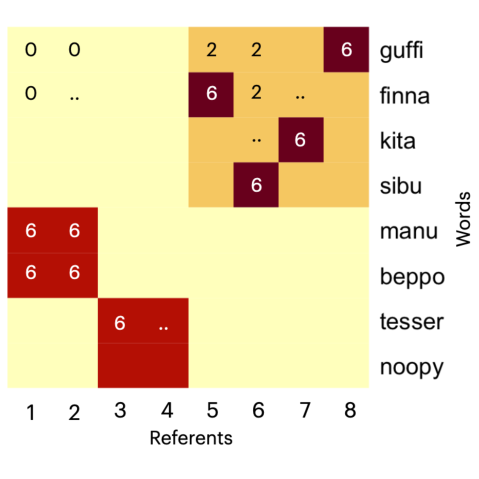
\includegraphics{figs/fig-exp-one-1} 

}

\caption[Word-referent co-occurrence matrix for Study (Experiment 1, Zettersten and Saffran, 2020)]{Word-referent co-occurrence matrix for Study (Experiment 1, Zettersten and Saffran, 2020).}\label{fig:fig-exp-one}
\end{figure}
\end{CodeChunk}

GK: we can also test this based on best-fitting model parameters:
``Intriguingly, we found that participants' sampling behavior was
correlated with their test accuracy: participants who chose more
ambiguous items during the Sampling Phase also more accurately
identified object-label associations. However, the directionality of
this correlation is unclear. One possibility is that learners were more
accurate on the test because they sampled more ambiguous items. Another
possibility is that success fully learning novel words during training
makes it more likely that learners will subsequently focus on ambiguous
items during the Sampling Phase. In the supplementary in-lab replication
experiment (see S1 for further details), we found preliminary evidence
supporting the latter explanation-- as participants become more
successful at learning the novel label-object associations, they also
become more likely to seek out information about ambiguous items.''

kids weren't more likely to sample the ambiguous referents: either they
are hypothesis testers (and saw no disconfirming evidence), or maybe
they have less of a focus on uncertainty (and perhaps slower learning
rate..and how does memory influence sampling choice? recency bias if
worse memory?)

\section{Method}\label{method}

\subsection{Data}\label{data}

All data were taken from @Zettersten2021. Data for our Study 1 were
pooled from Experiment 1 (31 adults), Experiment 2 (40 children, 4-9
years of age), and adults in the Ambiguous Condition of Experiment S1
(58 adults), which had the same design as Experiments 1 and 2, except
for an additional test before the selection phase.

The training phase of Study 1 contained 24 FixMe-second training trials,
each comprised of 2 referents and 2 words. The particular words and
referents involved in each pairing were randomized per participant, but
the same training trial sequence--and thus co-occurrence
statistics--were experienced by all participants. The accumulated
word-referent co-occurrences are shown in Figure 1.

Data for Study 2 come from Experiment 3, comprising 58 children, 3 to 8
years of age.

Selection trials for kids differ slightly from adults in that there was
no random label-referent pair given: thus, the evidence children
received after selection was unambiguous, while adults received a
training trial with a randomly-selected label and its corresponding
referent.

\subsection{Models}\label{models}

We focused on analyzing data from the familiarity- and
uncertainty-biased associative model
{[}@Kachergis2012,@Kachergis2017{]}, and variations of that model,
described below. We chose not to test any hypothesis-testing (HT) model
as they are not consistent with the adult data in @Zettersten2021: for
ambiguous items in the training phase, there was never any disconfirming
evidence, so a hypothesis-tester's initial guess (i.e.~hypothesis) for
each label would be confirmed on subsequent appearances, and there would
be no reason for (or basis for) preferentially selecting ambiguous
referents during the sampling phase, which is what adults were observed
to do. While it is possible that children -- who were at chance for
selecting ambiguous vs.~unambiguous referents -- are employing a
hypothesis-testing strategy, some of the selection strategies we want to
evaluate across development are only possible to use if a learner is
simultaneously entertaining multiple hypotheses for a given label --
equivalent to associations rather than the mutually-exclusive hypotheses
favored in HT accounts {[}e.g. @woodard2016{]}.

\subsubsection{Familiarity- and Uncertainty-biased Associative Model
(FUAM)}\label{familiarity--and-uncertainty-biased-associative-model-fuam}

The FUAM assumes that learners accumulate associations between all
presented words and referents on each trial, but that their attention is
biased more towards particular word-referent associations on the basis
of prior experience. In particular, more attention (i.e.~associative
weight) is directed to associations between words and referents that
have appeared together on earlier trials (i.e., a familiarity bias). In
addition, more attention is directed to stimuli that have higher
uncertainty (i.e.~entropy, \(H\)) in their associations, whether because
they are novel (and thus have no pre-existing associations) or because
they have diffuse associations with several different stimuli. The model
assumes learners knowledge grows trial-by-trial, and that a fixed amount
of associative weight (learning rate \(\chi\)) is distributed among the
presented word-referent associations on a given trial in proportion to
the prior familiarity of the association and the uncertainty of the
involved word and referent. The relative strength of the familiarity and
uncertainty bias is governed by a parameter \(\lambda\): for values of
\(\lambda>1\) the model focuses more attention on uncertain stimuli,
while for values of \(\lambda<1\) the model focuses more attention on
familiar word-referent associations. Associations are also assumed to
decay from trial to trial, at a rate governed by memory fidelity
parameter \(\alpha\). The update rule for adjusting the association
\(M_{w,o}\) between word \(w\) and referent \(o\) on a given trial is

\begin{equation}
M_{w,o} =  \alpha M_{w,o} + \frac{ \chi \cdot e^{ \lambda \cdot (H(w) + H(o)) } \cdot M_{w,o}  }{  \sum_{w\in W} \sum_{o\in O} e^{ \lambda \cdot (H(w) + H(o)) } \cdot M_{w,o} }
\label{eq:fullmodel}
\end{equation}

When tested on word \(w\), the model assumes learners choose referent
\(o\) from the offered alternatives in proportion to their associative
strength \(M_{w,o}\) (i.e., Luce choice).

The other models we tested are variations on this model.

\subsubsection{Familiarity-biased Associative Model
(FAM)}\label{familiarity-biased-associative-model-fam}

The familiarity-biased associative model (FAM) implemented just the
familiarity bias of the FUAM, without the uncertainty bias term, and
thus only implements a bias for already-strong associations, using
learning rate (\(\chi\)) and decay \(\alpha\) parameters.

\subsubsection{Uncertainty-biased Associative Model
(UAM)}\label{uncertainty-biased-associative-model-uam}

The uncertainty-biased associative model (UAM) implemented only the
uncertainty bias of the FUAM, without the familiarity bias term, and
uses the same three parameters as the FUAM.

\subsubsection{Novelty-biased Associative Model
(NAM)}\label{novelty-biased-associative-model-nam}

The novelty-biased associative model (NAM), like the UAM, has no
familiarity bias, but instead of the entropy terms (\(H(w)\) and
\(H(o)\)) uses novelty (e.g., \(1/(frequency(w)+1)\)).

\subsection{Fitting Procedure}\label{fitting-procedure}

We first fitted each model to each participant's data individually,
finding parameter values per participant to maximize the log-likelihood
of the model's choices with respect to theirs. We fitted each model to
just the passive training trials, as well as to the passive training
trials and the participant's selection trials, to confirm that including
the selection trials yielded a better fit. We will report each model's
average fit, and select the best-fitting model overall for further
analysis.

\subsection{Modeling Sampling Choices}\label{modeling-sampling-choices}

Next, we used the best-fit models of participants' learning to
investigate their selection strategies in the sampling phase of the
experiment. We considered three sampling decision rules commonly
attested in the information-seeking literature to explain active
choices: maximizing entropy reduction (information gain), maximizing the
probability associated with labels (probability gain), and margin
sampling.

\subsubsection{Maximizing entropy
reduction.}\label{maximizing-entropy-reduction.}

In this decision rule, the model's goal is to maximally reduce the
entropy of the object-label probability distribution across objects
{[}@Settles2012;@Nelson2005{]}. Sampling choices are modeled based on
comparing the relative entropy reduction provided by making a given
sampling selection of a referent \(s_o\) (across the labels \(w\)):

\begin{equation}
\max_{s_o,w}({H(w)-H(w|s_o)})
\label{eq:entropy_reduction}
\end{equation}

Modeling selections were made by determining, on any given trial for a
participant, which object maximally reduced entropy (averaging across
all possible random distractors that could be chosen in the case of the
adult data).

\subsubsection{Margin sampling.}\label{margin-sampling.}

An alternative strategy documented in describing active sampling
strategies is focusing on reducing uncertainty for a more constrained
set of items {[}@markant\_self-directed\_2016{]}. This strategy can be
formalized as \emph{margin sampling}, in which the model focuses only on
the boundary between two alternative options. Margin sampling predicts
that learners will focus on instances where there is highest ambiguity
between the two most likely labels for a given referent. Formally, if
the distribution of labels (\(\{l_1,l_2,...,l_n\}\)) for a given
referent \(o\) are ordered from most (\(p_1\)) to least (\(p_n\))
likely, \(\{p_1,p_2,...,p_n\}\), the margin between labels is given by

\begin{equation}
LM(x) = 1 - (p_1 - p_2)
\label{eq:margin_sampling}
\end{equation}

In other words, the model selects the object that has the greatest
ambiguity or competition between its two strongest associates.

\subsubsection{Maximizing probability
gain.}\label{maximizing-probability-gain.}

In this decision rule, the model's goal is to maximally increase the
probability associated between a random label and its object
{[}@nelson\_experience\_2010{]}. Selection choices are modeled based on
determining the increase in (correct) association strength provided by a
each potential object selection. The final object was selected that led
to the largest increase in association strength (averaging across all
possible distractors that could be chosen in the case of the adult
data).

\begin{equation}
\max_{s_o,w}({M_{w,s_o})- \max_{w,o}(M_{w,o}})
\label{eq:probability_gain}
\end{equation}

\subsubsection{Alternative strategies.}\label{alternative-strategies.}

We also explored several additional strategies. First, we also
considered a \emph{maximum certainty} (or confirmatory) strategy.
Learners may gravitate towards confirming choices they already have high
certainty for {[}@wason1960; @zettersten\_active\_2023{]}. Second, we
considered a \emph{novelty-based} strategy in which the model based its
choices on the relative novelty (or familiarity) of the choice options.
Third, we consider a random selection strategy as a baseline comparison.

\section{Results}\label{results}

\begin{table}[H]
\centering
\begin{tabular}{lrrrrr}
  \hline
Model & N best fit & strength & uncertainty & novelty & FUAM \\ 
  \hline
FUAM &  67 & 1.66 & 1.66 & 1.65 & 1.42 \\ 
  strength &  24 & 2.00 & 2.09 & 2.00 & 2.00 \\ 
  novelty &   3 & 3.22 & 3.42 & 3.01 & 3.19 \\ 
  uncertainty &  96 & 3.56 & 2.57 & 3.49 & 3.37 \\ 
   \hline
\end{tabular}
\end{table}

For all four models, including the selection trials yielded a better fit
to the data, showing that it is not unreasonable to apply these models
to the selection trials, and supporting the idea that the model's
knowledge state and parameters may bear some relation to participants'
selection strategies. For model comparison, we calculated BIC (Bayesian
Information Criterion), defined as \(BIC=ln(N)k-2ln(L)\), where \(L\) is
the maximized likelihood, \(k\) is the number of parameters, and \(N\)
is the number of data points (here, \(N=1712\) test trials). The model
with the lowest BIC is selected, as it balances model complexity and fit
to the data. The strength-biased model yielded \(BIC = 1036.17\), the
novelty-biased model scored \(BIC = 1026.68\), and the familiarity- and
uncertainty-biased model (FUAM) had \(BIC = 975.22\). The
uncertainty-biased model (UAM) yielded the best fit, with
\(BIC = 859.09\). Recognizing that different participants may be
operating under different learning regimes, we opted to investigate how
many participants were best fitted by each model. The uncertainty-biased
model best matched behavior of 96 of the 190 participants (51\% of the
sample), and the average fit (negative log-likelihood; see Table 1) of
the model to its best-fitted participants was much better (i.e.~lower)
than any other model (2.57 vs.~3.37 by the FUAM model). The FUAM
achieved the best fit for 67 participants, with the best average fit to
that group seen in Table 1 (1.42). The FUAM also matched the best fit of
the strength-biased model to 3 decimal places (see Table 1) for the 24
participants that were best fitted by that model, making for a total of
91 participants (48\% of the sample) that are best or nearly equally
well accounted for by the FUAM model (the uncertainty model did not fit
as well to the strength participants). The novelty-biased model best
fitted only 3 participants, although it's worth noting that its average
fit to the strength participants was nearly the same as the FUAM and
strength models. We will focus our remaining analyses on the model
parameters for the two best-fitting models, the familiarity- and
uncertainty-biased associative model (FUAM) and its cousin the
uncertainty-biased associative model (UAM).

\subsection{Model parameters}\label{model-parameters}

The FUAM and UAM models achieved similar fit
(\(|NLL_{FUAM} - NLL_{UAM}| \leq 0.1\)) for 98 participants. The UAM
achieved better fit than the FUAM (\(NLL_{FUAM} - NLL_{UAM} > 0.1\)) for
56 participants, and the FUAM achieved better fit than the UAM for the
remaining 36 participants. We will call these participants the
\emph{Either}, \emph{UAM}, and \emph{FUAM} groups, respectively.

\begin{table}[H]
\centering
\begin{tabular}{lrrrrr}
  \hline
Group & N & chi & lambda & alpha & Mean accuracy \\ 
  \hline
Either &  98 & 0.32 & 5.34 & 0.77 & 0.59 \\ 
  FUAM &  36 & 0.41 & 4.97 & 0.77 & 0.65 \\ 
  UAM &  56 & 0.26 & 8.76 & 0.69 & 0.57 \\ 
   \hline
\end{tabular}
\end{table}

Table 2 shows the average parameter values for each group of
participants, and the mean accuracy and number of participants per
group. None of these values are strikingly different than the overall
average parameter values (mean \(\chi=\) 0.32, mean \(\lambda=\) 6.28,
mean \(\alpha=\) 0.75), though the UAM group shows lower learning rate
(\(\chi = 0.26\)), lower memory fidelity (\(\alpha=0.69\)), and a higher
focus on uncertainty (\(\lambda=8.76\)). The FUAM group has a somewhat
higher learning rate (\(\chi = 0.41\) and the greatest overall accuracy
(\(M_{acc} = 0.65\)).

Figure 1 shows the correlations between participants' accuracy,
best-fitting model parameters, and log(age). All correlations are
significant (e.g., \(\lambda\) vs log(age) \(r = 0.14\),
\(t(187) = 1.99\), \(p<.05\)) except \(\lambda\) vs.~\(\chi\). Most
notable is that accuracy is strongly related to higher learning rate
\(\chi\) (\(r=0.53\)) and lower memory fidelity (\(\alpha=0.58\); better
learning is achieved by forgetting early, ambiguous evidence), and only
weakly related to \(lambda\) (\(r=0.23\)) and age (\(r=0.29\)). A
targeted analysis found that children (age\textless18) are more likely
than adults to be familiarity-focused (\(\lambda<1\)) rather than
uncertainty-focused (\(\chi^2 = 7.41\)): of 22\% of adults had
\(\lambda<1\), while 41\% of children did.

\begin{CodeChunk}
\begin{figure}[tb]
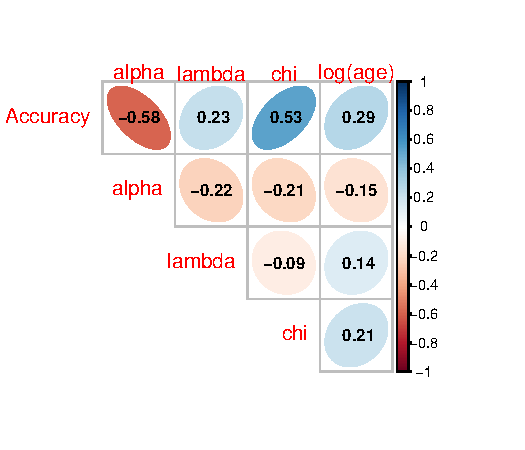
\includegraphics{figs/unnamed-chunk-2-1} \caption[Correlation of best-fitting model parameters]{Correlation of best-fitting model parameters}\label{fig:unnamed-chunk-2}
\end{figure}
\end{CodeChunk}

\begin{CodeChunk}
\begin{figure}[H]

{\centering 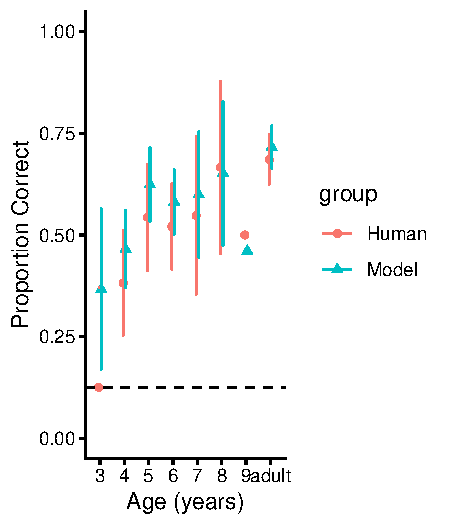
\includegraphics{figs/fig1-perf-1} 

}

\caption[Model vs]{Model vs. human performance by age.}\label{fig:fig1-perf}
\end{figure}
\end{CodeChunk}

\begin{CodeChunk}
\begin{figure}[H]

{\centering 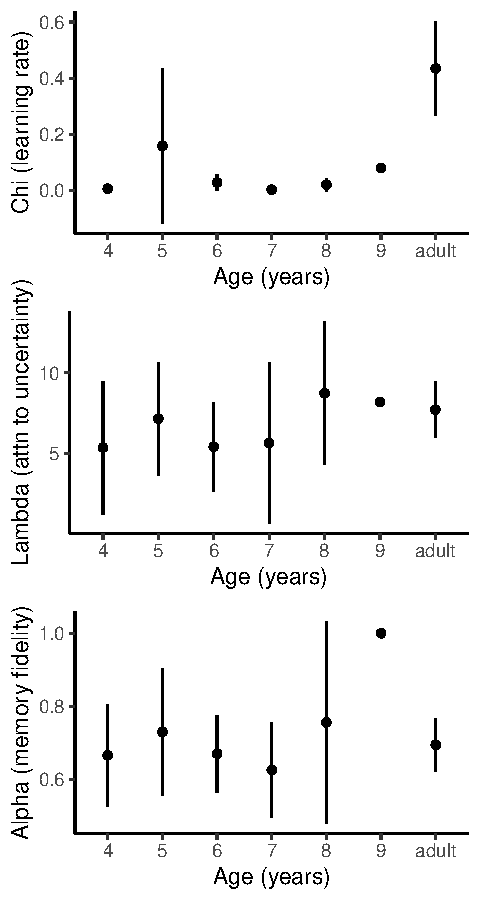
\includegraphics{figs/fig2-parms-1} 

}

\caption[One column image]{One column image.}\label{fig:fig2-parms}
\end{figure}
\end{CodeChunk}

\subsection{Selection Strategies}\label{selection-strategies}

The most likely selection strategy for each participant was calculated.
Confirmatory was the most common strategy (42\% of participants),
followed by entropy (29\%), margin sampling (18\%), random (8\%), and
novelty (3\%). Adults were more likely to use entropy maximization (39\%
vs.~20\% of children), whereas children were more likely to use a
confirmatory strategy (62\% vs.~22\% of adults). Margin sampling was
used at a similar rate by children (14\%) and adults (22\%), and a
random selection was most likely for 13\% of adults, but only 3\% of
children. Novelty was the most likely strategy for 5\% of adults, and no
children.

\begin{table}[H]
\centering
\begin{tabular}{lrr}
  \hline
strategy & n & proportion \\ 
  \hline
confirmatory &  81 & 0.42 \\ 
  entropy &  56 & 0.29 \\ 
  margin &  34 & 0.18 \\ 
  random &  15 & 0.08 \\ 
  novelty &   5 & 0.03 \\ 
   \hline
\end{tabular}
\end{table}

\begin{CodeChunk}
\begin{figure}[tb]
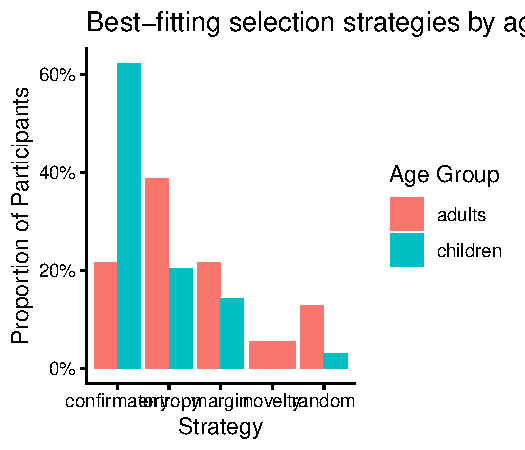
\includegraphics{figs/unnamed-chunk-5-1} \caption[Best-fitting selection strategies by age group]{Best-fitting selection strategies by age group.}\label{fig:unnamed-chunk-5}
\end{figure}
\end{CodeChunk}

\section{Discussion}\label{discussion}

\section{Acknowledgements}\label{acknowledgements}

Place acknowledgments (including funding information) in a section at
the end of the paper.

\section{References}\label{references}

\setlength{\parindent}{-0.1in} 
\setlength{\leftskip}{0.125in}

\noindent

\bibliographystyle{apacite}


\end{document}
